%% $RCSfile: proj_proposal.tex,v $
%% $Revision: 1.4 $
%% $Date: 2017/10/06 02:55:50 $
%% $Author: kevin $

\documentclass[11pt, a4paper, twoside, openright]{report}

\usepackage{float} % lets you have non-floating floats


\usepackage{url} % for typesetting urls

\usepackage{tikz} % for drawing diagrams
\usetikzlibrary{arrows.meta, positioning, shapes.geometric, shadows.blur}
\usepackage{pgfgantt} % for timeline gantt chart
\usepackage{pgfplots}
% \pgfplotsset{compat=1.18}

\usepackage{amsmath}
\usepackage{hyperref}
\usepackage{microtype}

\usepackage{todonotes}  % for adding todo notes REMOVE BEFORE FINAL

%  We don't want figures to float so we define
%
\newfloat{fig}{thp}{lof}[chapter]
\floatname{fig}{Figure}

% cfigure command:
% Usage: \cfigure[placement]{filename}{caption}
% - placement (optional): LaTeX float placement like htbp (default ht b p)
% - filename: the figure file name located inside the 'figures/' directory
% - caption: caption for the figure
\newcommand{\cfigure}[3][htbp]{%
   \begin{figure}[#1]
      \centering
      \includegraphics[width=0.8\textwidth]{figures/#2}
      \label{fig:#2}
      \caption{#3}
   \end{figure}%
}
%% These are standard LaTeX definitions for the document
%%
\title{Project title not yet defined}
\author{James Thompson}

%% This file can be used for creating a wide range of reports
%%  across various Schools
%%
%% Set up some things, mostly for the front page, for your specific document
%
% Current options are:
% [ecs|msor|sms]          Which school you are in.
%                         (msor option retained for reproducing old data)
% [bschonscomp|mcompsci]  Which degree you are doing
%                          You can also specify any other degree by name
%                          (see below)
% [font|image]            Use a font or an image for the VUW logo
%                          The font option will only work on ECS systems
%
\usepackage[,ecs]{vuwproject} 

% You should specifiy your supervisor here with
\supervisor{Ali Knott}
% use \supervisors if there are more than one supervisor

% Unless you've used the bschonscomp or mcompsci
%  options above use
\otherdegree{Master of Artificial Intelligence}
% here to specify degree

% Comment this out if you want the date printed.
% \date{}

\begin{document}

% Make the page numbering roman, until after the contents, etc.
\frontmatter

%%%%%%%%%%%%%%%%%%%%%%%%%%%%%%%%%%%%%%%%%%%%%%%%%%%%%%%

\begin{abstract}
  This is also undecided at this time and will be filled in later.
\end{abstract}

%%%%%%%%%%%%%%%%%%%%%%%%%%%%%%%%%%%%%%%%%%%%%%%%%%%%%%%

\maketitle

\tableofcontents

% we want a list of the figures we defined
%\listof{fig}{Figures}

%%%%%%%%%%%%%%%%%%%%%%%%%%%%%%%%%%%%%%%%%%%%%%%%%%%%%%%

\mainmatter

%%%%%%%%%%%%%%%%%%%%%%%%%%%%%%%%%%%%%%%%%%%%%%%%%%%%%%%

\listoftodos

\chapter{Introduction}

\todo[inline]{Unsure if this is needed. Yet could be a simple "one pager" (which is bigger than the one paragrapher of the abstract) that introduces the topic area, motivates the project and outlines the project.}

AI systems are on a trajectory to become more ingrained and operate more autonomously in our society. As these systems —currently LLMs— will increasingly make more decisions that effect human lives it is crucial that these systems are aligned with and reflect the values of the people they serve. What is being built could be your plumber, your lawyer or your doctor tomorrow what kind of being do you want these systems to be?

\chapter{Background}
\todo{Rethink the structure of the background chapter. Possibly reorder it}

\section{Large Language Models}

\subsection{Language models}

\textit{Language models are designed to understand and generate text. Generally probabilistic models that learn to predict next tokens. Use a large corpus of text data to learn statistical patterns in language. Started with simple statistical models such as n-grams and evolved to neural network based models such as RNNs, LSTMs and transformers.}

\subsection{Modern Large language models}

\textit{Modern LLMs are transformer based. Just use the decoder. Take the input and generate a sequence of tokens autoregressively. Use self attention mechanism to capture long range dependencies in text. Trained using next token prediction objective on large datasets.
Explain what self attention is (highlevel), how the basic architecture looks (layers of attention, feedfoward, multihead). How generation is done auto regressively. Lastly the training objective of next token prediction and very large corpus of text.}

\subsection{Applications of LLM}

\textit{LLMs are used a lot in modern day. Can achieve a lot. Agentic behavior is common.}

\section{Alignment of Large Language Models}

\subsection{What is alignment?}

As discussed above large language models (LLMs) have shown remarkable capabilities in understanding and generating human-like text. However the pre-training process focuses primarily on predicting the next token in a sequence, this does not necessarily mean that the model will produce useful, safe outputs that align with what users want. Therefore, aligning LLMs is generally \footnote{Other methods are proposed which embed the alignment within the pre-training step itself. Commonly used methods include filtering the training token} the process of taking the pre-trained model and fine-tuning it to better match what the designers and end users expect from the model. The aligning process can work on many dimensions of the models behavior from helpfulness, politeness, honesty, and safety to more complex values such as fairness, inclusively, and ethical considerations. More powerful models have a greater potential to cause harm if not properly aligned, making alignment along the dimensions such as safety and ethical considerations increasingly important. In this section I will outline some of the most common methods for post-training alignment of large language models along with current limitations and other methods.

\subsection{Alignment through preference optimization}
A common element in most post-training alignment methods is the use of preference optimization. The idea is to use a dataset of prompts and potential responses that are ranked either by humans or AI models to indicate which responses are preferred over others. This preference data is then used to fine-tune the pre-trained language model to increase the likelihood of generating preferred responses and decrease the likelihood of generating dis-preferred responses. With the goal that the final model will learn to generalize the preferences to new prompts and situations.

The distribution of prompts in the preference dataset is crucial as it defines the context for which the model is expected to generalize its learned preferences. Therefore it important to ensure that the prompts used to create the preference dataset are sufficiently representative of the contexts and dimensions in which you are expecting the model to align its behavior. Furthermore the rankings of the responses is also important as they define what the model is aligning towards. In many cases these rankings are subjective and provided by a small group of human labelers (n~50).
TODO: Expand this to explain the idea of generalization of preferences more rigorously.

\textbf{Note:}
\textit{Some of these subsection below of specific alignment methods could be compressed into single subsections and only explain the ones that are most relevant to my final proposed method. For now I include the three papers that I have actually read, I expect to compress RLHF and DPO into a "Other alignment methods" subsection. If I use more modern methods such as CAI with KTO or ORPO then I can expand on those more.}

\subsection{Reinforcement Learning from Human Feedback}
Reinforcement Learning from Human Feedback (RLHF) \cite{ouyangTrainingLanguageModels2022} uses human labellers to create the preference dataset and then a reinforcement learning algorithm to optimize the model based on this feedback. This method popularized post-training alignment and was used to train InstructGPT which was smaller and better at following instructions compared to GPT-3 \cite{brownLanguageModelsAre2020, ouyangTrainingLanguageModels2022}.

\subsubsection{How does RLHF work?}

RLHF is separated into three distinct stages. Firstly is supervised fine-tuning (SFT) where a pre-trained language model is fine-tuned on a dataset of prompts and human written 'expected' responses to those prompts. The second step is collecting multiple responses from the SFT model to create a set of prompts and response then having human labelers rank these responses from best to worst. This ranked data is then used to train a preference model (PM) that can predict which of two responses is better aligned to human preferences. Finally the PM is used as a reward signal in the PPO \cite{schulmanProximalPolicyOptimization2017} RL algorithm to further fine-tune the SFT model and create the final RLHF model.

\subsubsection{Relevance}

The idea of using human feedback to help train machine learning models is powerful, although it is not new and was around in theory and concept for years beforehand \cite{christianoDeepReinforcementLearning2017}. The specific method of RLHF was widely adopted \cite{team2023gemini,baiQwenTechnicalReport2023,shaoDeepSeekMathPushingLimits2024} yet is now replaced with more effective methods to utilize human feedback such as Direct Preference Optimization (DPO) \cite{rafailovDirectPreferenceOptimization2024}.

\subsection{Direct Preference Optimization}

The idea presented in \cite{ouyangTrainingLanguageModels2022} introduces the concept of using human feedback to train large language models to be aligned to human preferences. However the process of RLHF is complex and requires training multiple models (SFT, PM, RLHF). Direct preference optimization (DPO) \cite{rafailovDirectPreferenceOptimization2024} is a method that simplifies this process by removing the need for reinforcement learning altogether. Instead DPO reformulates the preference modelling step to instead create an objective function that implicitly creates the reward function from the model and a reference model (usually the SFT model).

\subsubsection{How does DPO work?}

DPO starts with the same preferences data as RLHF; a set of prompts with responses ranked by humans. Like RLHF it starts with a pre-trained language model and is supervised fine-tuned on the prompts and highest ranked responses to create an SFT model. Instead of training a separate preference model, DPO uses the SFT model and the current model to create the DPO update gradient:
\begin{equation*}
\begin{aligned}
\nabla_\theta \mathcal{L}_{\mathrm{DPO}}(\theta)
&= -\mathbb{E}_{(x, y^+, y^-) \sim D} \big[ \\
&\quad
\underbrace{
\sigma \!\left(
\hat{r}_\theta(x,y^-)
-
\hat{r}_\theta(x,y^+)
\right)
}_{\text{Reward model correctness}}
\left(
\underbrace{
\nabla_\theta \log \pi_\theta(y^+|x)
}_{\text{Increase preferred likelihood}}
-
\underbrace{
\nabla_\theta \log \pi_\theta(y^-|x)
}_{\text{Decrease dispreferred likelihood}}
\right)\\
&\big]
\end{aligned}
\end{equation*}

Where $\hat{r}_\theta(x,y) = \log \pi_\theta(y|x) - \log \pi_{SFT}(y|x)$ is the reward function defined as the log difference between the current model and the SFT model, $\sigma$ is the sigmoid function, and $(x, y^+, y^-)$ are the prompt, preferred response, and dis-preferred response respectively. \cite{rafailovDirectPreferenceOptimization2024} found that the reward model correctness weighting term for the update is very important. This update can be calculated with only 4 forward passes through the network per preference pair (2 for reference model and two for current model), making it much more efficient than RLHF \footnote{RLHF will need to do many forward passes of the network to train the preference model, then it will still have to do 3 forward passes for each datapoint when it comes to the RL step.}.

\subsubsection{Relevance}

DPO provides a more effective way to utilize the same underlying feedback data that is used in RLHF. It replaced RLHF as the baseline method for post-training alignment. Due to its widespread adoption DPO represents a strong baseline for alignment.

\subsection{Kahneman-Tversky Optimization}

\cite{ethayarajhKTOModelAlignment2024} sets out to change the objective of a language model to maximize the utility of generations as opposed to maximizing the log-likelihood of preferences. This introduces the concept of Human-aware losses (HALOs) which previous methods like DPO are. \cite{ethayarajhKTOModelAlignment2024} propose a new objective function from the HALO family that works on only binary preference data. This means rather than needing a prompt and at-least two responses (preferred and disprefered), you only need a single response and it will either be desirable response or undesirable response.

\subsubsection{How KTO works}

KTO is built off the foundation of prospect theory \cite{tverskyAdvancesProspectTheory1992} where the human utility of an random situation is determined by a value function and a weighting function. The value function is what determines how good/bad an outcome is compared to a reference point, and the weighting function is used to weight particular outcomes in a biased way in line with how humans perceive probability. KTO translates this theory into an objective function that uses binary preference data and a modified value function. It only needs a database of prompts and responses labelled as either desirable or undesirable ($d=1$ for desirable, $d=-1$ for undesirable). The KTO loss function is defined as:

\begin{equation*}
\mathcal{L}_{\mathrm{KTO}}(\pi_\theta, \pi_{\text{ref}}) = \mathbb{E}_{(x, y, d) \sim D} \left[ \lambda(d) - v(x,y)\right]
\end{equation*}
\noindent where
\begin{equation*}
\begin{aligned}
v(x,y) &=\begin{cases}
\lambda_D \sigma(\beta(r_\theta(x,y)-z_0)), & \text{if } d = 1 \\
\lambda_U \sigma(\beta(z_0 - r_\theta(x,y))), & \text{if } d = -1 \\
\end{cases}
\\
\lambda(d) &=
\begin{cases}
\lambda_D, & \text{if } d = 1 \\
\lambda_U, & \text{if } d = -1 \\
\end{cases}
\\
r_\theta(x,y) &= \log \pi_\theta(y|x) - \log \pi_{\text{ref}}(y|x)\\
z_0 &= D_\text{KL} \left( \pi_\theta(y|x) \| \pi_{\text{ref}}(y|x)\right)
\end{aligned}
\end{equation*}
The three  hyperparameters $\beta$ is a temperature parameter, and $\lambda_D$, $\lambda_U$ are scaling parameters for desirable and undesirable responses respectively. In the references implementation and experiments $\lambda_D = \lambda_U = 1$ and the reference model is a SFT model.

\subsubsection{Relevance}

Collecting the ranked preference data which is needed by normal alignment methods is normally quite expensive \cite{casperOpenProblemsFundamental2023} where binary like dislike information is much more natural and less invasive to collect. KTO is shown to be more efficient and more robust to data imbalances than DPO. Furthermore a model of sufficient size (~13B) does not need a SFT step prior to KTO which greatly reduces computational requirements. Furthermore KTO shows similar performance without using a reference model \footnote{This is done by assuming that the reference model returns a uniform distribution across all outputs given $x$} which also halves the memory requirements when training. 

\subsection{Constitutional AI}

\subsubsection{What is Constitutional AI?}

Constitutional AI (CAI) is a method of post-training a large language model to be aligned to set of principles that are outlined in simple natural language document called a constitution \cite{baiConstitutionalAIHarmlessness2022}. Importantly it works without the need for human labelling of data common in other alignment methods such as RLHF and DPO \cite{ouyangTrainingLanguageModels2022, rafailovDirectPreferenceOptimization2024}. Instead of human labelling CAI uses the model itself to generate feedback on its outputs based on the principles outlined in the constitution, this feedback is then used to further train the model to align it to the constitution.

\subsubsection{How does Constitutional AI work?}

CAI is a process that takes in a constitution, a pre-trained language model, and a dataset of prompts and outputs a model that is aligned to the constitution. The process consists of three main steps: self generative and supervised fine-tuning (SFT), preference modelling (PM), and reinforcement learning with human feedback (RLHF) \cite{baiConstitutionalAIHarmlessness2022}. The constitution itself was generated in an adhoc manner by the authors of \cite{baiConstitutionalAIHarmlessness2022} and consists of a set of principles that aim to make the model's outputs more helpful, honest, and harmless.

\begin{figure}[h!]
\centering
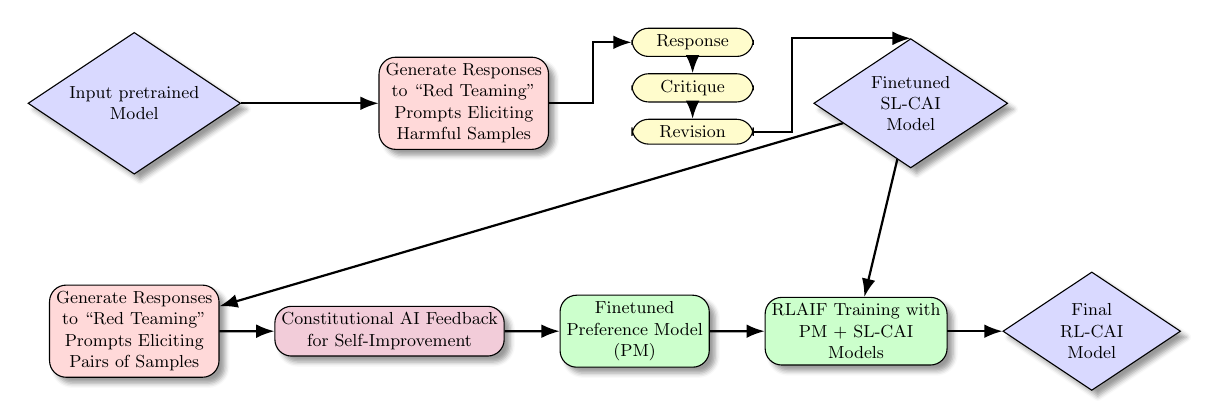
\begin{tikzpicture}[
    scale=0.7, transform shape,
    node distance = 2cm and 2.5cm,
    every node/.style={font=\small},
    diamond/.style={draw, shape=diamond, aspect=1.5, align=center, fill=blue!15, blur shadow},
    rect/.style={draw, rectangle, rounded corners=6pt, align=center, fill=red!15, blur shadow},
    smallrect/.style={draw, rectangle, rounded corners=6pt, align=center, fill=yellow!20, minimum width=2.2cm},
    process/.style={draw, rectangle, rounded corners=6pt, align=center, fill=green!20, blur shadow},
    stage/.style={draw, rectangle, rounded corners=6pt, align=center, fill=purple!20, blur shadow},
    arrow/.style={-Latex, thick}
]

% Top left diamond
\node[diamond] (input) {Input pretrained\\Model};

% Harmful sample generation
\node[rect, right=of input] (redteam1) {Generate Responses\\to ``Red Teaming''\\Prompts Eliciting\\Harmful Samples};

% response critique revision boxes
\node[smallrect, above right=0cm and 1.5cm of redteam1] (resp) {Response};
\node[smallrect, below=0.3cm of resp] (crit) {Critique};
\node[smallrect, below=0.3cm of crit] (rev) {Revision};

% SL-CAI diamond
\node[diamond, right=4.8cm of redteam1] (slcai) {Finetuned\\SL-CAI\\Model};

% Lower left harmful pairs
\node[rect, below=2cm of input] (redteam2) {Generate Responses\\to ``Red Teaming''\\Prompts Eliciting\\Pairs of Samples};

% constitutional AI feedback
\node[stage, right=1cm of redteam2] (cai) {Constitutional AI Feedback\\for Self-Improvement};

% preference model
\node[process, right=1cm of cai] (pm) {Finetuned\\Preference Model\\(PM)};

% RL-AIF model block
\node[process, right=1cm of pm] (rlaif) {RLAIF Training with\\PM + SL-CAI\\Models};

% final RL-CAI
\node[diamond, right=1cm of rlaif] (final) {Final\\RL-CAI\\Model};

% arrows
\draw[arrow] (input) -- (redteam1);

\draw[arrow] (redteam2) -- (cai);
\draw[arrow] (cai) -- (pm);
\draw[arrow] (pm) -- (rlaif);

\draw[arrow] (slcai) -- (rlaif);
\draw[arrow] (slcai) -- (redteam2);
\draw[arrow] (rlaif) -- (final);

% arrows from critique-response-revision group
\draw[arrow] (redteam1.east) -- ++(0.8,0) |- (resp.west);
\draw[arrow] (resp) -- (crit);
\draw[arrow] (crit) -- (rev);
\draw[arrow] (rev.east) -- ++(0.7,0) |- (slcai.north);

\end{tikzpicture}

\label{fig:cai_process}
\caption{Overview of Constitutional AI process, adapted from \cite{baiConstitutionalAIHarmlessness2022}}
\end{figure}

\subsubsection{Supervised learning on revised responses}

The first stage of the process involves taking the pre-trained model and using it to generate responses to a set of prompts. These prompts are designed to elicit harmful behavior. As the pre-trained model is designed to be helpful it will likely generate harmful responses to these prompts. These responses are then critiqued by the model itself using principles outlined in the constitution, only a subset of which are used for each response critique. The critique is then used to revise the original response to make it more aligned to the constitution. This process of generating responses, critiquing them, and revising them is done iteratively to create a dataset of revised responses. This dataset is then used to fine-tune the pre-trained model using self-supervised learning to create a model called the SL-CAI model.

\subsubsection{Reinforcement learning with AI feedback}
The next step involves using the SL-CAI model to generate pairs of responses to a set of prompts (overlapping with the set of prompts from before or not). Then using the constitution the SL-CAI model is used to provide feedback on which of the two responses is better aligned to the constitution. This feedback is then used to fine-tune a preference model (PM) that can predict which of two responses is better aligned to the constitution. Finally the PM and SL-CAI models are used together to do reinforcement learning in style of RFHL \cite{ouyangTrainingLanguageModels2022} to generate the final model RL-CAI. This final model is now aligned to the constitution without any human labelling of data. In the setup used in \cite{baiConstitutionalAIHarmlessness2022} the authors did in fact use some labels from human labelers which were used to provide the helpfulness signal in the preference model training, however in principle the preference signal could have been entirely generated by an AI model.

\subsubsection{Relevance}

In the context of when this paper was released there was a key dilemma of helpfulness vs harmlessness in large language models. Therefore, this paper set out to make a model that is both helpful and harmless, without sacrificing one for the other. Further research has expanded the horizons to be concerned with more than just harmfulness vs helpfulness trade off. As hinted at by the authors in \cite{baiConstitutionalAIHarmlessness2022}, there is room for improvement in the CAI method to make it focus on more than just harmlessness vs helpfulness. This can be done by modifying the constitutions to include more diverse principles as well as modifying the red teaming prompts to target more diverse scenarios (i.e controversial topics, political leanings, etc). In this way we can see how elements of CAI can be built upon by generating these diverse constitutions and red teaming prompts in a representative manner to create models aligned to a representative set of values.

\subsection{Current technical alignment limitations}

\textit{Introduce some of the ongoing concerns around current alignment methods. Such as shallow alignment, inner misalignment, scalable oversight etc.}


\section{Broader AI safety concerns}

\textit{
    Take the problem of alignment and expand it broader AI alignment concerns.
    Talk about mis generalization, and specification gaming.
    Introduce the concepts from PublicAI, incentives and collective intelligence.
    ...
}

\section{Representing Human Values}

\textit{
    Discuss concepts such as how does one understand the values of a group. How does it relate to building AI systems. I need to significant reading on this as I am most outside my comfort zone for this.
    Look into some philosophical concepts around how the collective the best baseline if we have no other gold standard. Provide some rationale as to why using the public as the source of values is a good idea, as opposed to some "gold standard" values provided by experts.
}


\chapter{Project Proposal}

\section{What I will do}

The goal of this project is to develop, implement and evaluate for future feasibility a method for aligning large language models to a set of representatively collected human values. This will be an end-to-end project that involves using current survey data and collecting new data, aligning a large language model using different methods and evaluating the effectiveness of the alignment.

\section{What problem I will solve}

Current methods for training large language models involve scraping the internet for large amount of text data. This creates a very powerful next token prediction model. Then to turn this models into something useful for the end user (e.g. chatbots, assistants, robo doctor etc) the model is aligned to how we want it to behave. Current methods for alignment involve contracting human labelers/annotators/demonstrators to provide data to give to the model on how we want it to behave. Problematically this is a opaque process that gives the end user little insight into what the model is "designed to do". Instead we can let the public directly and indirectly decide on what values they want the model to be aligned to. More so the public as the users and recipients of the model's outputs should have a say in the way that the model behaves. Large language models are on track to become tomorrows, accountants, lawyers, doctors and more, we need to ensure that we the people are the ones who decide on what kind of people they are.

\section{Timeline}

\todo[inline]{For now I will leave the timeline uncompleted. Once I have a more concrete idea of the method I will fill this in properly. There is code left in to help with how to make a gantt chart.}

The project will be carried out over three main phases. The first phase will be the organization and clustering of existing survey data to represent human values. The second phase will be an iterative process of aligning a large language model and evaluating its performance. The third phase involves collecting specific alignment data to further refine and train the model, followed by a final evaluation.

\begin{figure}[h!]
\centering
\begin{ganttchart}[
  vgrid, hgrid,
  x unit=0.5cm
]{1}{21}

  % --- Month labels ---
  \gantttitle{Jan}{2}
  \gantttitle{Feb}{4}
  \gantttitle{Mar}{4}
  \gantttitle{Apr}{4}
  \gantttitle{May}{4}
  \gantttitle{Jun}{3} \\

  % --- Week numbers ---
  \gantttitlelist{1,...,21}{1} \\

  % --- Work packages ---
  \ganttgroup{Survey Data Analysis}{1}{3} \\
  \ganttbar{Get access to data}{1}{1} \\
  \ganttbar{Organise \& Cluster Data}{2}{3} \\

  \ganttgroup{Aligning Model}{4}{18} \\
  \ganttbar{Select Base Model}{4}{4} \\
  \ganttbar{Pilot fine tune to test pipeline}{5}{6} \\
  \ganttbar{Full fine tuning runs}{9}{10} \\
  \ganttbar{Fine tuning with collected data}{17}{18} \\
  
  \ganttgroup{Evaluating Alignment}{7}{20}\\
  \ganttbar{Create Eval Method}{7}{9} \\
  \ganttbar{Initial Evaluation}{11}{12} \\
  \ganttbar{Final Evaluation}{19}{19} \\

  \ganttgroup{Public consultation}{13}{17} \\
  \ganttbar{Design}{13}{15} \\
  \ganttbar{Collect Responses}{16}{17} \\

  \ganttgroup{Writing report}{1}{21} \\
  \ganttbar{Writeup survey data clustering}{3}{3} \\
  \ganttbar{Writeup alignment process}{9}{10} \\
  \ganttbar{Writeup Eval method}{10}{11} \\
  \ganttbar{Writeup public consultation}{17}{17} \\
  \ganttbar{Complete writeup}{19}{21} 
\end{ganttchart}

\caption{Project timeline in weeks (only roughly aligned to months). This assumes a start time of end of January 2026 with near part time work ramping up to full time work by end of February.}
\end{figure}

\section{Output}

The output is both qualitative and quantitative in nature. There are four main deliverables:

\begin{itemize}
    \item A collection of aligned LLMs with various checkpoints of just survey data and then with the collected data.
    \item A public dataset of collected data around preferred values and responses for alignment.
    \item Experimental results evaluating the effectiveness of different alignment methods using the collected data.
\end{itemize}

\section{Resources needed}

There are two resource requirements for this project, hardware and public survey responses.

\subsection{Hardware}
The first is hardware which will be needed to do the alignment finetuning evaluation of the models. For the base LLM I would want to use a model in the range of 7 billion to 30 billion parameters, as this will get me close to state of the art performance on many tasks. This means that I will need access to about 200GB of GPU memory to be able to finetune the model effectively. Each finetuning run will take in the realm of 3-6 hours depending on the size of the model, amount of data used, alignment methods used and GPU hardware. Therefore given the goal of trying a handful of methods and different value sets I estimate about \footnote{4 hours per fine tune * 3 different methods * 5 different value sets + 5 hours of evaluation = 65 hours} 70 hours of GPU time will be needed. The cost of a GPU hour on a high end GPU such as a B200 is 6 USD per hour which would make the total cost about 420 USD.
Alternatively the Engineering and Computer Science department's GPU servers should give me access to machines with around 80GB of vram. This would allow me to fine-tune smaller models in the 7-13 billion parameter range. This should still be sufficient for a proof of concept and evaluation of the alignment methods.

\subsubsection{Public consultation responses}

The idea of using the public to help align large language models is central to this project. Most of the fine tuning will be done using the survey data which can be used to get the model roughly aligned to human values. However to get more specific and granular alignment I will collect new data from the public to further refine the model's behavior. This will be in the form of an interactive survey where participants will provide some form of preference feedback on model outputs. I envision using a tool like Polis or similar to collect and aggregate responses in a meaningful way. I would expect to need at least 50 or so people from the various subgroups and for each of them to spend maybe 2-3 15 minutes blocks providing feedback on model outputs.


%%%%%%%%%%%%%%%%%%%%%%%%%%%%%%%%%%%%%%%%%%%%%%%%%%%%%%%
\backmatter
%%%%%%%%%%%%%%%%%%%%%%%%%%%%%%%%%%%%%%%%%%%%%%%%%%%%%%%

%\bibliographystyle{ieeetr}
\bibliographystyle{acm}
\bibliography{references}
\end{document}
